%=======================================================================
% Copyright (c) 2012 The University of York and Willink Transformations.
%
% $Id: icmt13_52.tex 4506 2013-02-12 16:45:23Z hhoyos@CS.YORK.AC.UK $
%=======================================================================
\documentclass{llncs}
%
\usepackage{makeidx}  % allows for indexgeneration
\usepackage{listings}
\usepackage{graphicx}
\usepackage{multicol}
\usepackage{upquote}

%
\begin{document}
\lstdefinelanguage[omg]{ocl}
{morekeywords={and,body,context,def,derive,else,endif,endpackage,false,if,implies,in,init,inv,invalid,let,not,null,or,package,post,pre,self,static,then,true,xor},
sensitive=false,
morecomment=[l]{--},
morecomment=[s]{/*}{*/},
morestring=[b]",
}

%\lstdefinelanguage
%[[dialect] ] {language}
%[ [base dialect]{hand base languagei} ]
%{key=value ... }
%[ [hlist of required aspects (keywordcomments,texcs,etc.)i] ]
\lstdefinelanguage{qvtc}
[omg]{ocl}
{morekeywords={import,transformation,imports,uses,map,in,refines,check,enforce,where,realize,default,query},
}
\lstset{
basicstyle=\scriptsize,
tabsize=4,
% Numbering
numbers=left, numberstyle=\tiny, numbersep=5pt}

\mainmatter              % start of the contributions
%
%\title{Towards an extended family of QVT languages}
\title{QVT Imperative - A practical semantics for declarative transformations}
%
\author{Horacio Hoyos \and Dimitris Kolovos\inst{1} \and Edward Willink\inst{2}}
%
\institute{The University of York, York, UK,\\
\email{horacio.hoyos.rodriguez@ieee.org, dimitris.kolovos@york.ac.uk},\\
\and
Willink Transformations Ltd., Reading, UK \\
\email{ed@willinktransformations.co.uk}}

\maketitle              % typeset the title of the contribution

%=======================================================================
% Copyright (c) 2012 The University of York and Willink Transformations.
%
% $Id: abstract.tex 4481 2013-02-12 14:15:46Z hhoyos@CS.YORK.AC.UK $
%=======================================================================
\begin{abstract}
%using at least 70 and at most 150 words.
%The early enthusiasm that led to the definition of the QVT specification for the standardization of model transformation languages subdued due to the lack of an industrial quality implementation. 
% 1)The early enthusiasm (2002) for model to model transformation languages led to eight submissions (2003) for an OMG standard (2007) comprising three languages; no commercial products have appeared (2013).


% The problem is not the lack of an industrial quality.  The problem is that the lack of an industrtail quality implementation of the QVT languages has stopped QVT
%The problem is that
%Initial enthusiasm around the QVT specification has subdued and a hybrid declarative/imperative a commercial product is still missing and available implementations do not provide the complete set of QVT languages. 

The early enthusiasm, in 2002, for model to model transformation languages led to eight submissions for an OMG standard comprising three languages, yet no commercial products have appeared. The QVT Core language was intended as the foundation for QVT Relations but the available implementations have ignored the core language. Rather than ignoring the core language, we take the opposite approach and introduce three more core languages. Progressive program-to-program transformation through these core languages terminates in an easily implemented imperative language that supports declarative transformations.

% Optionally add a fifth sentence being positive about progressing from ATL, sharing knowledge, tooling etc.

%Initial enthusiasm around the QVT specification has subdued evidenced by the lack of a commercial product implementation; further, available implementations only provide support to QVTr (Relations) or QVTo (Operational Mappings). In fact, there are no QVTc (Core) implementations although the QVTc language was intended as the common foundation for QVTr and QVTo. To provide a complete QVT implementation that delivers the hybrid declarative/imperative facilities required by model transformations we expand the QVT alphabet to six languages. The additional languages are a semantic subset of QVTc; they bridge the semantic gap between highly declarative QVTr relations and a low level imperative operations. Additionally, they provide interchange points at different levels of abstraction that serve as interface points for other transformation languages, with the intention to promote knowledge sharing and collaboration. 

%Our additional core languages are semantic subsets of QVTc; they define important interchange points during the progressive program-to-program transformation from a highly declarative QVTr program via QVTc to a low level imperative program.



% QVTc (Core) was intended as the common foundation for QVTr (Relational) and QVTo (Operational Mappings) and due to its simpler semantics 
 %have not implemented the QVTc (Core) language. The lack of a QVTc implementation that can be used as an engine for QVTr (Relations) transformations
  %simpler semantics of QVTc, its implementation should be simpler and it can then be used semantics of the QVTr (Relations) 
%The simpler semantics of QVTc suggest that its implementation should be simpler In the QVT specification the QVTc language s  and QVTo (Operational Mappings) implementation

%As Eclipse QVTo and Medini QVTr projects stall a set of QVT parallel initiatives emerge, such as ATL, Kermeta and ETL, that due to their lack of standardization fail to create and reuse common knowledge, increasing the engineering and development cost.
%"As Eclipse QVTo and Medini QVTr projects stall a set of QVT parallel initiatives emerged, such as ATL, Kermeta and ETL, leading to fragmentation and duplication of effort in the Model Transformation community."
% 2) The QVTc (Core) language was intended as the common foundation for QVTr (Relational) and QVTo (Operational Mappings); the available implementations ignore the core language. 
% This is aproblem becuase QVTc was inteded as the common fundation for QVTr and QVTo. 
 
 
% The simplest way to implement QVT, addressing the semantic complexity of bidirectional model transformations, is to augment the QVT alphabet so that a particular language provides suitability for a certain part of the complexity. 
 %3) It is clear that the three language compromise between declarative and imperative approaches was insufficient and so we expand the QVT alphabet to six languages.
 
 
% The implementation of the proposed subset of QVTc languages will allow QVTr transformations to be executed by providing the required semantics and offer standard interchange points for current and future model transformation language initiatives.
%4) Our additional core languages are semantic subsets of QVTc; they define important interchange points during the progressive program-to-program transformation from a highly declarative QVTr program via QVTc to a low level imperative program.







%Optionally add a fifth sentence being positive about progressing from ATL, sharing knowledge, tooling etc.


\keywords{QVT, OCL, virtual machine, program transformation, declarative transformation, progressive transformation, transformation chain}
\end{abstract}


%\input{Outline}

%=======================================================================
% Copyright (c) 2012 The University of York and Willink Transformations.
%
% $Id: introduction.tex 4512 2013-02-12 20:47:04Z hhoyos@CS.YORK.AC.UK $
%=======================================================================
\section{Introduction}
The importance and benefits of standardisation are widely recognised in all engineering disciplines. In the domain of Model Driven Engineering, the OMG has provided a set of standards related to modelling and model management. One of these standards is the Query/View/Transformation (QVT) specification\cite{QVT1.1} that addresses the task of model transformation. Although the QVT Request For Proposals (RFP)\cite{QVT-RFP}  in 2002 attracted 8 submissions, ten years later the initial enthusiasm has failed to mature into any commercial implementations.

The RFP called for one transformation language, but the submitters could not agree whether an  imperative or declarative approach should be used, and so a compromise between the two viewpoints was resolved by specifying three languages. Three languages might seem like a typical committee outcome, however in this paper we run with this compromise and start to argue for six languages.

The QVT Operational Mappings language (QVTo) supports an imperative form of model transformation and is the most successful with two Open Source implementations available; SmartQVT and the QVT Operational project at Eclipse. The most recent release of SmartQVT was in 2008. Eclipse QVTo was originally developed by Borland, and after a three year lull is again under active maintenance and development.

The QVT Relations (QVTr) language provides powerful multi-directional declarative transformation capabilities. It has two implementations. Medini QVT is Open Source, provides a partial implementation but does not appear to be progressing. Performance results have been very disappointing \cite{Bosems2011}. ModelMorf is proprietary but the freely available Beta releases have not matured into a product.

The QVT Core (QVTc) language provides much simpler multi-directional declarative capabilities. The internal submission prototype at Compuware was never updated to match the specification and so QVTc has never had an implementation.

At Eclipse, the QVT Declarative project has provided editors, parsers and models for QVTr and QVTc but no execution capability. This paper describes ongoing activity towards remedying the execution deficiencies.

The two-level declarative approach adopted by the QVT specification provides powerful abstractions but no obvious way to realize them. For efficient execution we want a highly optimized imperative representation that we call QVT Imperative (QVTi). Following the QVT specification's suggestion that QVTr should be realized by a program-to-program transformation to QVTc, we propose a program-to-program transformation from QVTc to QVTi. This transformation will be realized as a chain of three program-to-program transformations from QVTc via QVT Unidirectional (QVTu) and QVT Minimal (QVTm) to QVTi. In a future paper, we will discuss the QVTc to QVTi transformations and the QVTu and QVTm languages. In this paper, we concentrate on the QVTi semantics, its execution and the reuse of QVTc concrete syntax for QVTi (and QVTm and QVTu).

It should be noted that the QVT 1.1 specification failed to address any of the issues raised against QVTc in the QVT draft or 1.0 specification, and since no prototype of QVTc has been produced anywhere, we have to treat the precise wording of the QVT specification with a little scepticism. We therefore work to what we perceive to be the spirit rather than the letter of the specification. Our tooling introduces a QVTo-like import statement for the QVTc  metamodels, including the middle metamodel.

In this paper we present the motivation for the three new QVTc subset languages in section \ref{sec:motivation} and an overview of QVTc in section \ref{sec:qvtcore}. The details of QVTi are presented in section \ref{sec:qvti}, with related work presented in section \ref{sec:related}. Finally, section \ref{sec:concandfuture} concludes.

%=======================================================================
% Copyright (c) 2012 The University of York and Willink Transformations.
%
% $Id: subsetLanguages.tex 4326 2013-01-31 17:44:31Z hhoyos@CS.YORK.AC.UK $
%=======================================================================
\section{Motivation}\label{sec:motivation}
In QVTr, a model transformation is defined using powerful abstractions. A set of relations that \textquotedblleft declare constraints that must be satisfied by the elements of the candidate models\textquotedblright\cite{QVT1.1}.

\begin{itemize}
\item Constraints are defined by matching properties of elements in the candidate models.
\item Property matching uses expressions written in OCL and grouped in domains.
\item Each domain represents a candidate model.
\item Constraints can be specialized to check models (checking semantics).
\item Constraints can be specialized to modify models (enforcement semantics).
\item Constraints semantics varies with the chosen transformation direction.
\end{itemize}

The complexity of the language semantics, and the underlying abstractions of pattern matching, constraints and OCL make the specification and implementation of QVTr a complex and daunting task. The QVT specification uses an almost unreadable and untested QVTr to QVTc transformation to `solve' the problem.

QVTc is \textquotedblleft as powerful as the Relations language, though simpler. Consequently, the semantics of the Core Language can be defined more simply, though transformations described using the Core are more verbose\textquotedblright \cite{QVT1.1}. Since in QVTc the trace models must be explicitly defined, constraints are now defined by matching properties of elements in the candidate models and the trace models. Checking and enforcement provide the same functionality as in QVTr.

A QVTc transformation is specified as a set of mappings with constraints defined in a domain for each candidate and trace model. The simpler semantics of QVTc  make a QVTc implementation more tractable. QVTc makes only small abstract syntax extensions to EMOF and OCL. A QVTc implementation is therefore an attractive intermediate implementation approach for QVTr. This approach may use a debugged version of the QVTr to QVTc transformation from the specification.

However, multi-directional transformations still present several challenges in a number of domains and disciplines \cite{Czarnecki.etal2009}, some of which translate to QVT\cite{Stevens2010}. Declarative transformations present a challenge from a rule schedulability point of view. In the specific case of QVT this translates to an implementation in which the execution of rules can be partial, interrupted or postponed until matches in other rules provide the required variable values (bindings), eventually requiring multiple passes. These challenges can be overcome by removing multi-directionality, normalizing constraints and defining an imperative semantics. 

However, the semantic gap between \textless multi-directional + declarative\textgreater\hspace{0pt} and \textless uni-directional + imperative\textgreater\hspace{0pt} makes it difficult to tackle the aforementioned aspects in a one-step mapping. Moreover, there is a risk that what was gained from having to implement a simpler semantics would be lost by the work needed to realize the required mappings.

\begin{figure}[h]
	\centering
	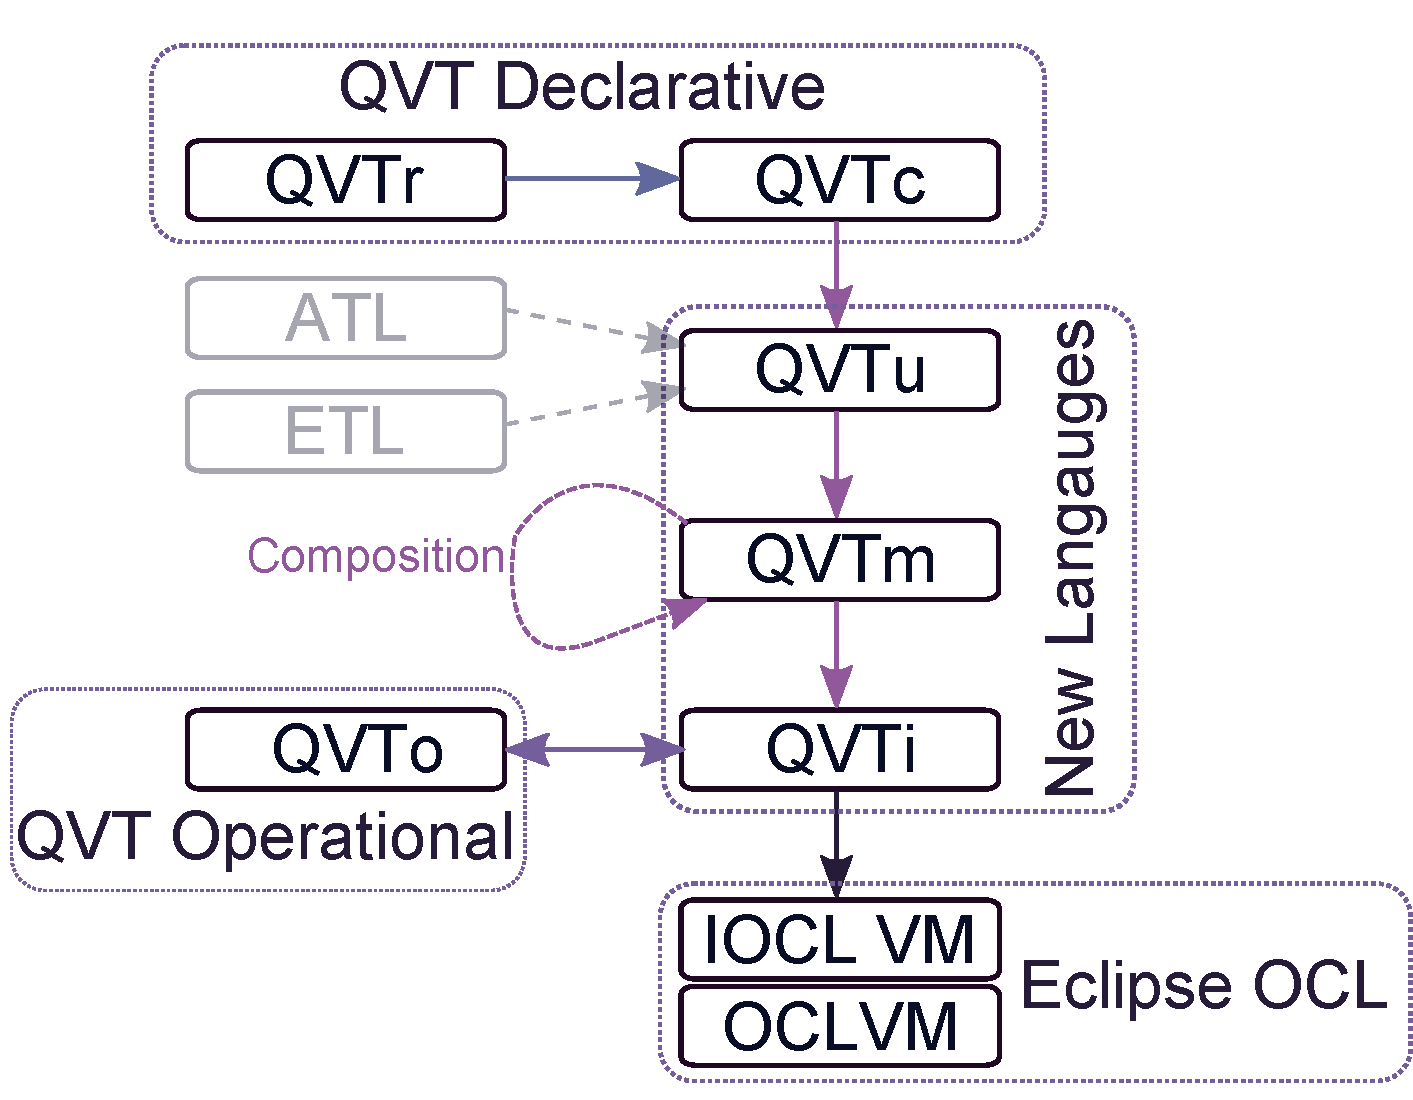
\includegraphics[width=0.56\textwidth]{QVTView.pdf}
	\caption{Overview of the proposed QVT 6 languages architecture.}
	\label{fig:overview}
\end{figure}

Figure \ref{fig:overview} presents our progressive transformation solution to realizing QVTr on an OCL Virtual Machine\cite{Willink2012}. At the top we have the two QVT Declarative languages, with QVTr realized by a QVTr to QVTc program-to-program transformation. Our three new languages, QVTu, QVTm and QVTi are syntactic and semantic simplifications of QVTc.

\begin{itemize}
\item For QVT Uni-directional (QVTu), we align the transformation to the user's invocation context and eliminate the redundant multi-directional and enforcement flexibilities.
\item For QVT Minimal (QVTm) we normalize to eliminate syntactic sugar and alternate representation flexibilities.
\item For QVT Imperative (QVTi) we discard declarative flexibilities and synthesize a multi-pass imperative search schedule that can be executed easily by a model-friendly Virtual Machine.
\end{itemize}

These new languages are not just a convenience for realizing QVTc, they also offer important interchange points for other transformation technologies to exploit and so share the tool chain.

\begin{itemize}
\item QVTu provides a high level interchange point for other uni-directional declarative transformation languages such as ATL or ETL.
\item QVTm provides a normalized representation at which declarative transformation composition and optimisation can be applied.
\item QVTi provides a low level interchange point that imperative transformation languages such as QVTo, ALF or EOL may exploit.
\end{itemize}

%three new languages, each one supporting a more restricted QVTc abstract syntax and providing increasingly limited semantics. QVTo operations will be invoked at the QVTi level and QVTi will provide an interface for QVTo to populate the middle (trace) model. Proximity of the QVTc abstract syntax to EMOF and OCL will be useful as an AST interpretation and execution can be provided by extending the Eclipse OCL Virtual Machine\cite{Willink2012}.

%The intention of the QVTc subset languages is then to progressively restrict the QVTc semantics to eventually define a subset of QVTc that is uni-directional, normalized and imperative. The different levels of semantic \textquotedblleft power\textquotedblright will also imply a restriction on the use of the language's abstract syntax, from permissive to restricted. An overview of the proposed QVT alphabet is presented in Figure \ref{fig:overview}. 

%Complete support for QVTr is achieved by specifying mappings and implementing automated program transformations for:
%\begin{itemize}
%\item  QVTr$\rightarrow$QVTc, written in QVTc
%\item  QVTc$\rightarrow$QVTu, written in QVTu
%\item  QVTu$\rightarrow$QVTm, written in QVTm
%\item  QVTm$\rightarrow$QVTi, written in QVTi
%\end{itemize}

%The first restriction is to remove bi-directionality, thus QVTu (unidirectional) restricts the semantics so that in the context of a mapping (the name given to rules in QVTc) only one candidate model can be enforced. The next restriction is to remove rule specialization, thus QVTm (minimal) does not allow mapping refinement. Finally, to remove the declarative component, in QVTi (imperative) mappings are allowed to introduce only one unbound variable and transformations must be written as a tree of mapping compositions were each root mapping declares the constraints between one of the candidate models and the trace model.  Execution of all the languages is provided by performing automated transformations from semantically richer languages to simpler ones, for example form QVTr to QVTc or from QVTm to QVTi.








%=======================================================================
% Copyright (c) 2013 The University of York and Willink Transformations.
%
% $Id: icmt13_52.tex 4326 2013-01-31 17:44:31Z hhoyos@CS.YORK.AC.UK $
%=======================================================================
\section{The QVT Core Language}\label{sec:qvtcore}
QVT Core (QVTc) is a surprisingly simple multi-directional, multi-input, multi-output declarative model transformation language. The complexities of multi-versatility are considered in \ref{Direction}. In the following description, we therefore consider just a simple left to right transformation.

A declarative model transformation language declares the many transformation relationships that all the objects in all the input models and in all the output models satisfy on completion of the transformation; it does not necessarily specify how this is achieved. The complexity of the many relationships is managed by exploiting the familiar metamodels, shown at the left and right hand sides of Figure \ref{fig:TransformationAnatomy}. These comprise packages and types to categorize the different kinds of objects in a model. The Transformation adds Mappings and Patterns to organize the different kinds of relationship to be satisfied.

\begin{figure}[h]
	\centering
	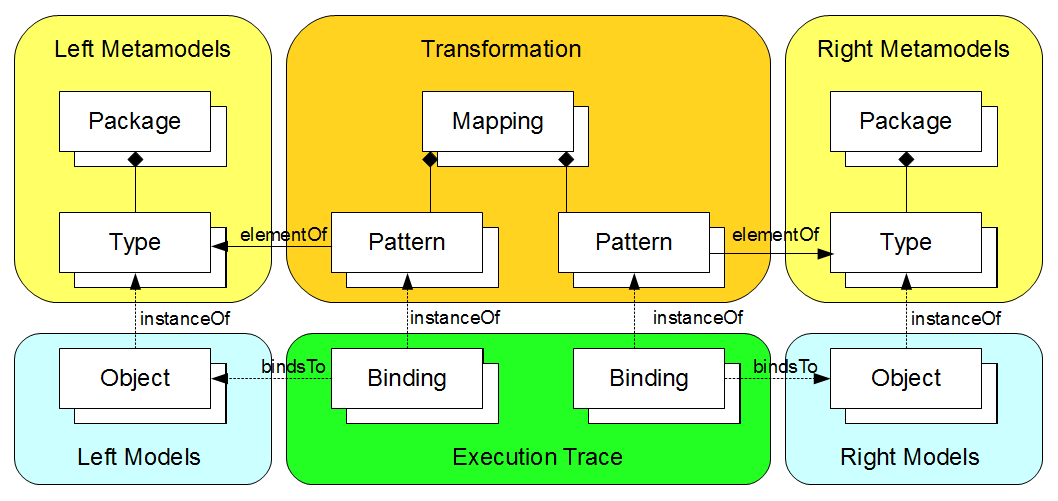
\includegraphics[width=0.8\textwidth]{TransformationAnatomy.png}
	\caption{Transformation Anatomy.}
	\label{fig:TransformationAnatomy}
\end{figure}


Figure \ref{fig:pattern} is an Object Diagram showing an example Pattern describing a parent-child match. The pattern involves two pattern variables \textit{theParent} and the \textit{theChild} each of which may be bound to a \textit{Node} object in a user model. The pattern imposes the additional constraint that the objects bound to \textit{theParent} and  \textit{theChild} variables must lie at each end of a \textit{parent}-\textit{children} Association. The \textit{theParent} lies at the composing (diamond) end of an optional (?) multiplicity.  The \textit{theChild} lies at the end of an arbitrary (*) multiplicity.

\begin{figure}[h]
	\centering
	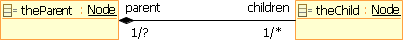
\includegraphics[width=0.7\textwidth]{pattern.png}
	\caption{Example Parent-Child Pattern.}
	\label{fig:pattern}
\end{figure}

When the transformation relationships are satisfied, the models have been partitioned into groups of objects and every object is a member of at least one group. Each group is identified by a Binding in which the Type of each object conforms to the Type of the Pattern element to which the object is bound. The interrelationships between the bound objects similarly conform to the interrelationships between the pattern elements. For the example pattern, each Binding comprises a pair of \textit{Node}s one bound to \textit{theParent} and the other bound to \textit{theChild}. A Binding exists for every possible pair of \textit{Node} objects that match the Pattern. The transformation between the Bindings is defined by Mappings, each of which defines the interrelationships between one left Pattern and one right Pattern.


The foregoing principles are common to many declarative and some imperative transformation languages. It is in the way in which mappings are structured that transformation languages vary.

\subsection{Traceability and the Middle Model}
A significant challenge for model transformation arises in specifying how the overlap of output Bindings is to be handled. A common solution provides specialized constructs to interrogate the execution trace and so allow the instantiation of one Pattern to interact with the instantiation of another. These specialized constructs are often rather obscure. QVTc is unusual in making the traceability model explicit; it is called the Middle model. Figure \ref{fig:QVTCoreAnatomy} shows how for QVTc there are three Domains, Left, Middle and Right, each of which comprises Models and Metamodels. Associated with each Domain are the Bindings and Patterns.

\begin{figure}[h]
	\centering
	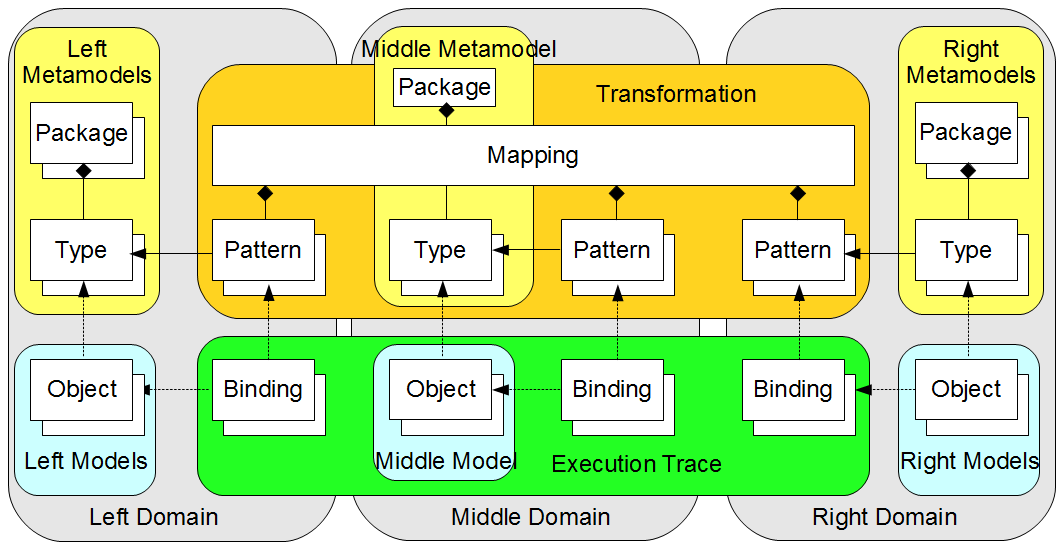
\includegraphics[width=0.9\textwidth]{QVTcore.png}
	\caption{QVT Core Anatomy.}
	\label{fig:QVTCoreAnatomy}
\end{figure}

The additional Middle model may be quite simple and the Middle Bindings may be free from overlap. This may significantly simplify the transformation exposition since with the aid of the intermediate, a direct N:M mapping from left-to-right may be expressed as a two-pass transformation comprising an N:1 left-to-middle pass and a 1:M middle-to-right pass. Any information that needs to be gleaned from the left can be cached in the middle model during left-to-middle pass so that it is readily available for use during the middle-to-right pass. Very complex transformations may specify additional passes that operate from Middle model to Middle model.

The Middle model of course conforms to its metamodel and, for QVTc, it is the transformation author's responsibility to design the Middle metamodel so that overlaps can be resolved and information cached. %[The more powerful QVTr language, when implemented by a QVTc engine, requires the Middle metamodel to be synthesized as part of the QVTr to QVTc program to program transformation.]

\subsection{Intra-Mapping Semantics}

Within a Mapping, the QVTc semantics are simple; each Domain comprises a GuardPattern and a BottomPattern. The GuardPattern is responsible for the matching, and the BottomPattern for the model mutation. 

\begin{figure}[h]
	\centering
	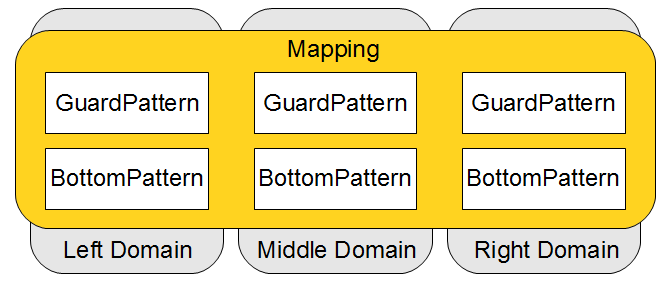
\includegraphics[width=0.5\textwidth]{QVTcoreAreas.png}
	\caption{QVT Core Areas.}
	\label{fig:QVTCoreAreas}
\end{figure}

The two-dimensional layout shown in Figure \ref{fig:QVTCoreAreas} is difficult to achieve in a text file and so the concrete syntax is

{\scriptsize \begin{verbatim}
map {
  left  ( left-guard-pattern-variables | left-guard-pattern-constraints )
        { left-bottom-pattern-variables | left-bottom-pattern-constraints }
  right ( right-guard-pattern-variables | right-guard-pattern-constraints )
        { right-bottom-pattern-variables | right-bottom-pattern-constraints }
  where ( middle-guard-pattern-variables | middle-guard-pattern-constraints )
        { middle-bottom-pattern-variables | middle-bottom-pattern-constraints }
}
\end{verbatim}}

Let us consider a very simple example of a bidirectional transformation between colored Node trees with different color representations; HSV (hue, saturation, value) on the left, HLS (hue, lightness, saturation) on the right and RGB (red, green, blue) as a middle intermediate. Figure \ref{fig:TreeMM} shows the three metamodels with the additional traceability references from middle metamodel to the external metamodels.  Listing \ref{lsting:QVTcExample} presents the QVTc transformation for this example.

\begin{figure}[hb]
	\centering
	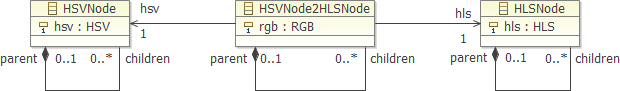
\includegraphics[width=0.95\textwidth]{Metamodels.png}
	\caption{Simple colored Tree metamodels; Left(HSV), Middle(RGB), Right(HLS).}
	\label{fig:TreeMM}
\end{figure}

\input{qvtc.lst}

Lines 1 to 15 provide some boilerplate; the \texttt{import} statements of the actual metamodels whose package names are the same as the file name; the \texttt{transform\-ation} declaration including an unnamed \textit{TypedModel} for the middle model; declarations of the color converter queries whose definition is omitted for space reasons.

Lines 16 to 28 provide the \textit{Node2Node} mapping, without any guard variables or constraints; the mapping is therefore unbound. Each domain realizes a \textit{Node}, and so requires that where that node exists in an input domain, the corresponding nodes are created or updated in the middle and output domains. Lines 21 to 24 initialize the middle node from whichever of \textit{hsv} or \textit{hls} is the input and lines 25 to 26 initialize the color value of the \textit{hsv} or \textit{hls} nodes from the middle node.

Lines 30 to 38 refine the \textit{Node2Node} mapping to enforce consistency at the root so that all root nodes have no parent. Lines 40 to 47 refine the \textit{Node2Node} mapping to enforce consistency of parent-child relationships. The guard pattern introduces an additional parent node variable for each domain and requires that this is indeed the parent of each node inherited from \textit{Node2Node}. For the input domain, the parent-child relationship is interpreted as a guard, whereas for the middle and output domains, the parent-child relationship is enforced.

The foregoing quick summaries demonstrate how the combination of the pattern variable declarations, some of which can be realized while others must exist, and the assignments of OCL queries to properties support symmetrical definition of multi-directional transformations. Some declarations are distinct for each direction, others adopt distinct predicate or assignment semantics according to the transformation direction.

% In each domain we are interested in two elements (the parent and the child), so we need two pattern variables to capture the two parts of a Binding. These variable are constrained, firstly by their type, secondly by an explicit constraint that the two nodes have the same color and finally by an explicit constraints that one fulfills the relation of being the parent of the other. A naive transformation tool may just iterate each variable over each model element to identify each candidate binding and then prune those that fail to satisfy all constraints. A slightly more intelligent tool may iterate only over the model elements that conform to the required type. For this trivial example all model elements are of the same type so a type check achieves little. For more realistic metamodels the basic type constraint should significantly reduce the mantissa of an exponential computation cost. A much more intelligent tool should exploit the metamodel relationships so that at most the first pattern variable involves a full model search; subsequent variables can be searched for locally. In our example, after choosing a parent candidate, only its children need consideration. Careful use of the metamodel to plan search strategies can reduce the naive exponential complexity to something much closer to linear for many practical problems.

% Returning to the QVTc exposition. The GuardPattern orchestrates the search, so in the GuardPattern we declare the two pattern variables with their constraining types and provide the additional matching color constraint. Once the GuardPattern has been satisfied, the BottomPattern provides the copy of the selected child from left to right.

% Our example loses information and so cannot be executed in reverse. However we can still examine the example to understand the symmetries that QVTc provides. In the forward direction, an assignment defines the valid right hand output from left inputs. Conversely for a reverse transformation the forward assignment acts as a predicate rejecting candidate right hand elements that are inconsistent with the forward transformation. For example on Listing \ref{lsting:QVTcExample} if the transformation was executed in the direction of the \texttt{subTree} model, the predicate in line 21 will cause the \textit{color} attribute of \textit{\textbf{cT}} to be set to the value of the \textit{color} attribute of \textit{\textbf{pT}}. If we executed the transformation in reverse (i.e. in the direction of \texttt{coloredTree}) then the predicate in line 21 will act as a constraint evaluating that both elements have the same \textit{color}.

\subsection{Inter-Mapping Semantics}

A single mapping is of limited utility. Practical transformations require many mappings and an ability to share context between mappings. Consider a mapping from a hierarchical metamodel such as UML. A high level mapping may transform packages, and the transformed package is then needed as context for a mapping involving classes. QVTc supports independent mappings by declaring each as a top level mapping as in Listing \ref{lsting:QVTcExample}. Shared context is supported by declaring the dependent mappings as nested within the mapping whose bindings the nested mapping shares as in Listing \ref{lsting:QVTiExample}.

QVTc supports reuse of mappings within a transformation by refinement, and reuse of transformations by inheritance.

\subsection{Execution Modes}

\subsubsection{Direction}\label{Direction}

The multi-directional capability allows a single QVTc transformation program to specify many model transformations, and to avoid the inconsistencies that may arise through writing independent programs for each direction and enforcement.

A multi-directional transformation does not have unambiguous inputs or outputs and so a QVTc transformation is specified between TypedModels. In practice only one direction will be of interest at any one time and so once the invocation identifies which TypedModels are inputs and which are outputs, a practical QVTc tool may optimize away the redundant declarations for unwanted directions. Since all transformations are not reversible, QVTc allows the programmer to restrict particular Domains to input or output by using the \texttt{check} or \texttt{enforce} keywords.

\subsubsection{Enforcement}\label{Enforcement}

A transformation may be used for more than one purpose: \textit{check}, \textit{update} or \textit{create}. In the more common case, a transformation \textit{creates} output models corresponding to input models. A transformation may also be used to \textit{check} that existing output models are consistent with input models, or to \textit{update} existing output models to be consistent with input models. In the case of an update, for many important system applications the update may need to occur in-place. For this use case, the declarative QVTc exposition enables the QVTc tooling to ensure that the update occurs in a coherent fashion so that all input locations are read before any co-located output locations are written.


%\input{subsetLanguages}

%=======================================================================
% Copyright (c) 2012 The University of York and Willink Transformations.
%
% $Id: QVTi.tex 5455 2013-05-17 10:15:50Z ed@willink.me.uk $
%=======================================================================
\section{The QVT Imperative Language}\label{sec:qvti}
The QVT Imperative (QVTi) language re-uses the principles and syntax of QVTc to provide an easily executable semantics that can be targeted by the program-to-program transformations shown in Figure \ref{fig:overview}, i.e., QVTi is intended to be a machine generated language rather than written by a programmer. The major simplifications of QVTi in comparison to QVTc are:
\begin{itemize}
\item Uni-directional (not multi-directional)
\item Specific creation/update/check behavior (no check/enforce flexibility)
\item No complex syntax such as refinement, or inheritance (no syntax sugar)
\item No mappings have both source and target domains (no complex dataflow)
\item Multiple mappings are executed sequentially (rather than declaratively)
\item Nested mappings may be invoked directly (rather than declaratively)
\end{itemize}

These simplifications combine to support a simple mode of execution in which mappings are executed in sequence within simple loops. Nested mappings nest in a manner that allows a conventional execution stack to maintain the prevailing state of each search variable. The overall transformation is executed as a guarded depth-first search of the source and then middle model spaces. Where the guarded search matches, either the middle model element temporarily persists the context of the match, or a target model element is updated.

The search strategy is defined by the program-to-program transformation that produces the QVTi program. As a minimum this producer must serialize mappings with multi-variable patterns so that sub-mappings re-use rather rediscover parent bindings. This serialization offers significant opportunities for optimization through the use of the known metamodels and optionally through profiling as well. It is very desirable for the search to iterate over easy navigation paths such as compositions and forward references. It is also desirable to search first over model elements that have strict guard conditions since these may result in early pruning of the search space. It is highly undesirable to perform whole model searches or traverse associations in an unnavigable direction. 

We will demonstrate the simplified QVTi semantics by reworking the Listing \ref{lsting:QVTcExample} example in accordance with a user requirement to create an HLS model from an HSV model. The resulting mappings, shown in Listing \ref{lsting:QVTiExample}, are manually produced pending future work on the program-to-program transformation chain.

\input{qvtiListings.lst}

%The major simplifying semantics of QVTi involves decomposing the mappings for multi-variable patterns into multiple sub-mappings each of which introduces exactly one new pattern variable. variables extension patterns so that the conversion to QVTu simplifies the transformation to support just creation of HLS from of HSV. The conversion to QVTm flattens the refinements. Then the conversion to QVTi imposes a multi-pass search schedule, one pattern variable at a time. The search schedule is carefully chosen to exploit the metamodels, so that successive steps use easily navigable paths and early pruning of the search space by evaluating constraints as soon as their pattern variables are bound. Total model searches and unnavigable paths are avoided wherever possible. 

The transformation starts with a potentially declarative match of the guard variable(s) of the first mapping to the `whole' model, from which  The \textit{GuardPattern} on line 2 of HSV2MiddleRoot selects the \textit{HSVNode} source without a parent.
%Since the transformation is now solely executed from \textit{hsv} to \textit{hsl}, the \texttt{check} and \texttt{enforce} keywords have been removed.
Where this  match is found, lines 5-7 realize an \textit{HSVNode2HLSNode} middle node and populate it with the source context and computed RGB value.

The two nested mapping calls on lines 10-17 are then executed sequentially. Explicit mappings calls are the sole extension in QVTi. The target mapping is invoked with the guard variable to the left of each \texttt{:=} assignment bound to the value of an OCL expression, and the guard variable to the left of each \texttt{<=} assignment looping over each value of the collection-valued OCL expression.

The \textit{HSV2MiddleRecursion} mapping is therefore invoked with its \textit{hsvNode} guard variable bound to each of the original source node's children, and its \textit{middleParent} bound to the realized middle node. The \textit{HSV2MiddleRecursion} realizes a corresponding middle node for each source node and recurses down the source tree.

Once the \textit{HSV2MiddleRecursion} completes, the \textit{HSV2MiddleRoot} mapping resumes and invokes the \textit{Middle2HLSRoot} mapping, binding its \textit{middleNode} guard variable to the \textit{middleRoot} node. The \textit{Middle2HLSRoot} behaves in a very similar fashion realizing a target node and using the \textit{Middle2HLSRecursion} to build the target tree.
%Notice in this case that since \textit{hls} is a target domain, the \texttt{enforce} keyword has been preserved.

This simple example demonstrates the simplifications underlying QVTi and the one syntax extension to QVTc. With these reduced semantics QVTi still has the power to express important programming idioms.
%In order to define this as a QVTc, rather than QVTi extension, we define the invocation on line 8, as providing bound search domains for the two guard variables of the \textit{HSV2MiddleRecursion} mapping named \textit{hsvNode} and \textit{middleParent}. Where collections are provided as the bound domains for non-collection guard variables, a distinct \texttt{mapping} invocation occurs for the Cartesian product of each variable from each bound domain. Guard variables not bound by the invocation are bound one element at a time to the whole model. This is a natural extension restricting the declarative search space of QVTc whereby every guard variable is bound to the whole model. For QVTi, we impose the reduced semantics that at most one bound domain may be a collection and no guard variables may be left unbound, thereby ensuring that the invocation involves at most a simple loop.


\subsubsection{Sequencing and Passes}
Sequential execution of multiple patterns within one pass or of multiple passes can be expressed by sequential nested mappings as in the \textit{HSV2MiddleRecursion} then \textit{HSV2MiddleRoot} sequencing.

\subsubsection{Iteration and Recursion}
Looping over multiple model elements is supported by a \textit{GuardPattern} variable bound to each element in turn of a collection of model elements as in the \textit{HSV2MiddleRecursion} over the children. Simple iteration loops may use nested \textit{mappings}. Recursive loops exploit a nested mapping that invokes a named mapping with bindings. This syntax extension short-circuits the total model search associated with a declarative exposition.  

\subsubsection{Conditional Execution}
Arbitrary OCL constraints may be used in the guards for each step of each iteration. The example is very regular so there is only a single `at the root' guard for the \textit{HSV2MiddleRoot} mapping.

\subsubsection{Model Mutation}
Model elements are created by the realized variable declarations in the bottom patterns. Arbitrary OCL queries define the value to be assigned to each model element, or the iteration domain of a nested mapping. These expressions appear to the right of \texttt{:=} or \texttt{<=} operators in the example.

\subsubsection{Traceability}
Traceability is provided by the middle model. This is user-defined and so allows the user to control how much information relating source and target is maintained. In a more complex example OCL expressions may navigate from source or target models to the middle model using the standard UML opposite navigation semantics.

\subsubsection{Timing}
Preparation of the optimized QVTi transformation as AST or compiled Java is a compile-time activity that may be performed ahead of time whenever the desired execution direction mode is also known ahead of time.


%QVTi is a very small unidirectional imperative transformation language that is syntactically a subset of QVTm.  The intention of QVTi is to allow imperative constructs to be written in QVTc. This means that transformations will explicitly define the order of execution of mappings by limiting the number of unbound variables to one and by using nested mappings to support common imperative programming idioms. The limited semantics allow that a minimal extension of the OCL VM\cite{Willink2012} can be implemented to provide QVTi support. Current development demonstrated that the IOCL (imperative OCL) VM presented in Figure \ref{fig:overview} is no longer needed as the \textit{Type.createInstance} and \textit{Property.initValue} in the current OCL API are enough to provide the side effects required to modify or create elements in the candidate and middle models.  The example introduced in section \ref{sec:qvtcore} is useful to understand the effects of the progressive semantic restrictions that are introduced when mapping QVTc to QVTu to QVTm to QVTi. Listing \ref{lsting:QVTiExample} presents the Node to subtree transformation written in QVTi. 
%: limited semantic bandwidth, if/switch/loop/seq/recurse/multi-pass idioms, minimal OCL VM change.

%As required in QVTu, lets assume the user selected the subtree model as the output and an enforcement operation mode. The effect of this selection is that all \texttt{enforce} keywords are removed from the input domains, i.e., domains which associated model type is \textit{coloredTree} (see lines 12 and 25). Consequently, \texttt{check} keywords are removed from output domains, i.e., domains which associated model type is \textit{subTree} (see lines 43 and 55). Since in the original QVTc transformations there aren't any refinements, composition of mappings is not required.

%Explicit order of execution is done by using nested mappings. Further, in QVTi execution order must follow a 3+ step sequence better described as:
%\begin{verbatim}%Z
%map {
%  map input-to-middle {...}
%  map middle-to-middle {...}
%  map middle-to-output {...}
%}
%\end{verbatim}
%Where several middle-to-middle mappings may be used. This is particularly useful for in-place transformations where the required information is first copied form the candidate model to the middle model and then used to create/update the candidate model. This guarantees that create/update operations do not affect \textit{checking} when the model is an input. Since there is a single root mapping and nested mappings are evaluated sequentially, there is only one execution order eliminating declarative execution. 

%The other key aspect of QVTi is the limit of 1 unbound variable per mapping, as this restriction is useful when using mappings to build common programming idioms as presented next.

%\begin{itemize}
%\item In the original QVTc transformations the mapping for the input model defined two variables. In QVTi, since only one unbound variable is allowed, the original mapping is rewritten as a mapping that defines \texttt{pHT:HueTree} (line 12) with a nested mapping in which \texttt{cHT:HueTree} is introduced (line 25). 
%\item A single variable introduced in a guard pattern is used to create an \textit{if} expression. This is the case of line 25-27 where \texttt{cHT:HueTree} is introduced but the MiddleBottomPattern and the nested map will only be evaluated if the \texttt{cHT.parent := pHT;} and \texttt{cHT.color := pHT.color;} conditions are met. Additionally, since the ColoredTree metamodel enumerates the possible colors, the set of possible values could be used to create a \textit{switch} statement by testing the cHT color attribute against a specific value , eg. \texttt{cHT.color := Color::red;}

%\end{itemize}


%Ideally the example should flow through so that the utility of the bulets is demonstrated

%The foregoing semantic limitations support the following programming idioms
%- sequential/nested execution
%- if/switch
%- loop iteration
%- recursion
%- multiple passes

%again one paragraph each with as much reuse of the example as possible


\subsection{Implementation}
Some simple QVTi transformations have been implemented using the Eclipse QVTi editor and parser and the Eclipse OCL VM\cite{Willink2012}.

The OCL VM offers two modes of execution, the simplest of which is interpreted. It comprises a simple tree-walking evaluator over the OCL AST. This evaluator is realized by an extensible EvaluationVisitor and so, since the QVTi AST is an extension of the OCL AST, it is sufficient to extend the OCL EvaluationVisitor to support the additional QVTi AST nodes.

This proved to be surprisingly easy. It was not even necessary to add extensions for model mutation since the Eclipse OCL VM has a prototype type constructor implementation.\footnote{Type constructors extend the Tuple syntax to allow construction of fully initialized user objects as e.g. \texttt{Person\{name:='Me'; age:=20;\}.}
}

The API provides only two methods to create objects and to initialize fields. These were sufficient for the disciplined form of model mutation in QVTi. 
%The extended IOCL VM with Imperative OCL functionality shown in  Figure \ref{fig:overview} has not been necessary for QVTi; it may yet prove necessary to fully integrate QVTo.

The Eclipse OCL VM also offers a tree-walking code generator that produces a direct Java realization of OCL. This has been extended to support the additional QVTi AST nodes and so generates direct Java code for a QVTi transformation. 

\subsection{Future Work}\label{Future Work}

We will now discuss a number of complexities that we have glossed over so far.

\subsubsection{Bootstrapping}

The QVT specification assumes the existence of a QVTr capability in order to realize the QVTr to QVTc transformation. We propose to provide partial implementations of the QVTr to QVTi chain using ETL/Flock\cite{Paige.etal2009}. These bootstraps will be promoted to QVTu using a further ETL/Flock to QVTu transformation (also using ETL/Flock). The final promotion from QVTu to QVTc or QVTr will be manual.

\subsubsection{Update/Check}

A transformation may create or update target models or just check source models. These distinct modes of execution are resolved at the same time as multi-directionality; the transformation relationships are adjusted to reflect that user's requirements. In the case of a check or update transformation a reconciliation of multiple source models is synthesized. The QVTi implementation is simplified by only needing to execute the single required mode of execution.

\subsubsection{In-Place Update}

A QVTc transformation is amenable to in place execution since the middle model separates the source and target model accesses. It is only necessary to ensure that the generated QVTi schedule caches source accesses in the middle model before any target updates introduce conflicts.

\subsubsection{Generality}

Declarative rule matches provide arbitrary flexibility without efficiency, whereas the imperative QVTi schedule provides efficient realization only of metamodel guided rule sequences. However QVTi retains the ability to perform a brute force recursion over all possible rules, so there is no loss of generality. The ongoing research goal is to maximize the ability to exploit the metamodel.

\subsubsection{Performance}

Once the QVTr to QVTc to QVTi program-to-program transformations are in-place, we can look forward to a high performance direct Java realization of QVTr. And with QVTr in-place, the slightly verbose expositions of the QVTc and its subset languages can be ignored by users. Only transformation toolsmiths need use them to exploit their interchange opportunities.

%What we do want is an inpractice section.

%The OCL capabilities have been reused without change. Mutation was already available through type constructor support provision of Type.createInstance() and Propery.initValue(). The IOCL VM of Fig 1 is therefore not needed for declarative, but may be need for QVTo.

%The OCL evaluator with its tree walking interpreter with (? 50 nodes) is easily extended for QVT Core where

%Transformation ...
%TypedModel is structural
%Mapping ...
%Domain ...
%GuardPattern ...
%BottomPattern ...
%...


\section{Related Work}\label{sec:related}

The Kermeta model transformation language development tools include code generators that can transform Kermeta transformations into Java and Scala code which can then be executed against a Java Virtual Machine (JVM) for more efficient execution \cite{Fouquet.etal2010}. The Epsilon\cite{Paige.etal2009} platform of model management languages also features a layered approach where all model task-specific languages extend a common expression language (EOL).

Following the paradigm of VM-based programming language architectures (e.g. JVM), the Atlas Transformation Language (ATL) features a layered architecture in which transformations are compiled to XML-based byte-code, which is then executed by a virtual machine \cite{Jouault.etal2008}. The architecture of ATL enables the substitution of the default VM with custom VM implementations. Beyond the default generic VM, ATL ships with an additional optimized VM for transforming EMF-based models. The ATL VM is based upon the ATL language and so has limited integration with its OCL implementation. The similarities of the QVT and ATL architectures provide interesting points for interoperability\cite{Jouault.Kurtev2006}. In contrast our approach exploits the inherent tree structure of the OCL AST to extend the Eclipse OCL VM's tree-walking interpreter and code generator for the extended QVTi AST. 

Building on the idea of a 2-stage execution of model transformations, in \cite{Wagelaar.etal2011}, the authors present a generic transformation engine VM (EMFTVM). Similarly to the ATL VM, EMFTVM also executes byte-code but unlike the ATL VM where byte-code is represented using proprietary XML, in EMFTVM byte-code conforms to an Ecore metamodel -- and as such it is easier for higher-level transformation languages to compile down to it using higher-order transformations. The aim of EMFTVM is to serve as an underlying VM for additional transformation languages and as a proof of concept, the developer of the EMFTVM has implemented higher-order model transformations that map transformations expressed both in ATL and in a simple graph transformation language\footnote{http://soft.vub.ac.be/soft/research/mdd/simplegt} to VM byte-code. The concept of a reusable EMF-based VM that can act as a compilation target for higher-level languages is similar to the approach proposed in this paper. However, in our approach we envision multiple hook points which will allow transformation languages operating at different levels of abstraction to integrate with the proposed architecture with reduced duplication.

The most similar approach to the one proposed in this paper, is the work presented in \cite{Sanchez-Barbudo.etal2008} where the authors propose a layered architecture for implementing QVTc and QVTo. More specifically, the authors propose a program-to-program transformation to compile QVTc and QVTo transformations into a low-level imperative transformation language called Atomic Transformation Code (ATC), and then compile ATC code to byte-code that can be executed by a proprietary virtual machine called Virtual Transformation Engine (VTE). The architecture of our approach is similar, but we propose to eliminate dependencies on proprietary components (ATC), and to further decompose the compilation process by introducing additional intermediate QVTx languages.


%\input{virtualMachine}

%=======================================================================
% Copyright (c) 2012 The University of York and Willink Transformations.
%
% $Id: icmt13_52.tex 4326 2013-01-31 17:44:31Z hhoyos@CS.YORK.AC.UK $
%=======================================================================
\section{Conclusions}\label{sec:concandfuture}

We have proposed a progressive program-to-program transformation chain from QVTr to QVTc to QVTu to QVTm to QVTi, in order to provide a simple unidirectional imperative language that provides a practical execution semantics for QVTc and QVTr. We have introduced the QVT Imperative (QVTi) language and presented its simple semantics and basic syntax. We have demonstrated that QVTi may retain the basic QVTc concrete syntax and yet support useful idioms for optimized pattern matching strategies and multiple passes. Our preliminary QVTi implementations demonstrate that the Eclipse OCL VM interpreter is easily extended for QVTi. We can therefore look to exploit the Eclipse OCL VM's Java code generator to provide good quality compiled Java code and then concentrate on the QVTc to QVTi program-to-program transformations to provide effective execution strategies.

%QVTu may be an appropriate entry point at which other declarative transformation languages such as ATL, Epsilon or Viatra2 reuse a shared transformation framework.


%
% ---- Bibliography ----
%
\bibliographystyle{splncs03}
\bibliography{hhr502References}

\end{document}